% ----------------------------------------------------------------
% AMS-LaTeX Paper ************************************************
% **** -----------------------------------------------------------
\documentclass[9pt]{amsart}
\usepackage{graphicx}
% ----------------------------------------------------------------
\vfuzz2pt % Don't report over-full v-boxes if over-edge is small
\hfuzz2pt % Don't report over-full h-boxes if over-edge is small
% THEOREMS -------------------------------------------------------
\newtheorem{thm}{Theorem}[section]
\newtheorem{cor}[thm]{Corollary}
\newtheorem{lem}[thm]{Lemma}
\newtheorem{prop}[thm]{Proposition}
\theoremstyle{definition}
\newtheorem{defn}[thm]{Definition}
\theoremstyle{remark}
\newtheorem{rem}[thm]{Remark}
\numberwithin{equation}{section}
% MATH -----------------------------------------------------------
\newcommand{\norm}[1]{\left\Vert#1\right\Vert}
\newcommand{\abs}[1]{\left\vert#1\right\vert}
\newcommand{\set}[1]{\left\{#1\right\}}
\newcommand{\Real}{\mathbb R}
\newcommand{\eps}{\varepsilon}
\newcommand{\To}{\longrightarrow}
\newcommand{\BX}{\mathbf{B}(X)}
\newcommand{\A}{\mathcal{A}}
% ----------------------------------------------------------------





\begin{document}

\title[YARP]{
YARP: Yet Another Ridiculous Paper}%
\author{IIT Robotics Lab}  %


%\keywords{manipulation, grasping, humanoid robotics, motion primitives}%

%\date{}%
%\dedicatory{}%
%\commby{}%
% ----------------------------------------------------------------
\maketitle
% ----------------------------------------------------------------
%\vspace{-0.9cm}
%\begin{center}
%{Robotics Behavioural \& Cognitive Sciences Lab\\ IIT, Italian Institute of Technology, ITALY}
%\end{center}
%\vspace{0.5cm}


\vspace{-0.2cm}
\begin{center}
{\emph{\textbf{Abstract}}}
\end{center}
\vspace{0.2cm}

\emph{In this paper we describe the actuation and control of a humanoid robot neck. Particular attention will be posed on the description of the neck actuation structure, the design of which results in a noticeable human similarity. Specifically, the final mechanical design was inspired by the human skeleton, with the neck bone movements constrained and actuated by the surrounding muscles. In our robotic platform, the neck bone was realized with a steel spring surrounded by steel tendons in place of muscles. The specific and innovative mechanical design have imposed the design of a non-standard actuation structure which, in turn, have lead to an innovative control scheme.} 




\section{Introduction}

Humans exhibit a wide and complex repertoire of movements far beyond the motor capabilities of modern robots. Clearly, the
realization of an artificial system capable of more realistic movements passes trough a series of technological improvements,
especially if we are interested in replicating both kinematic and dynamical aspects. Recently, there has been a growing interest in developing robots whose geometric and actuation structures resemble those of a human being. Probably, one of the most extreme steps in this direction is represented by the robot recently developed by O. Holland and colleagues \cite{Cronos}; another interesting example is the humanoid robot Kotaro \cite{Kotaro}.


\section{Humanoid platform} \label{Sec:Platform}

The robotic platform on which the discussed controllers have been implemented is the humanoid robot James \cite{James06}.\\James is a 22-DOF torso with moving eyes and neck, an arm and a highly anthropomorphic hand. In the following subsections we briefly cover the robot design, its actuation, and sensorization. More details about the neck structure are given in section 3.

\begin{figure}[h!tbp]
\centering
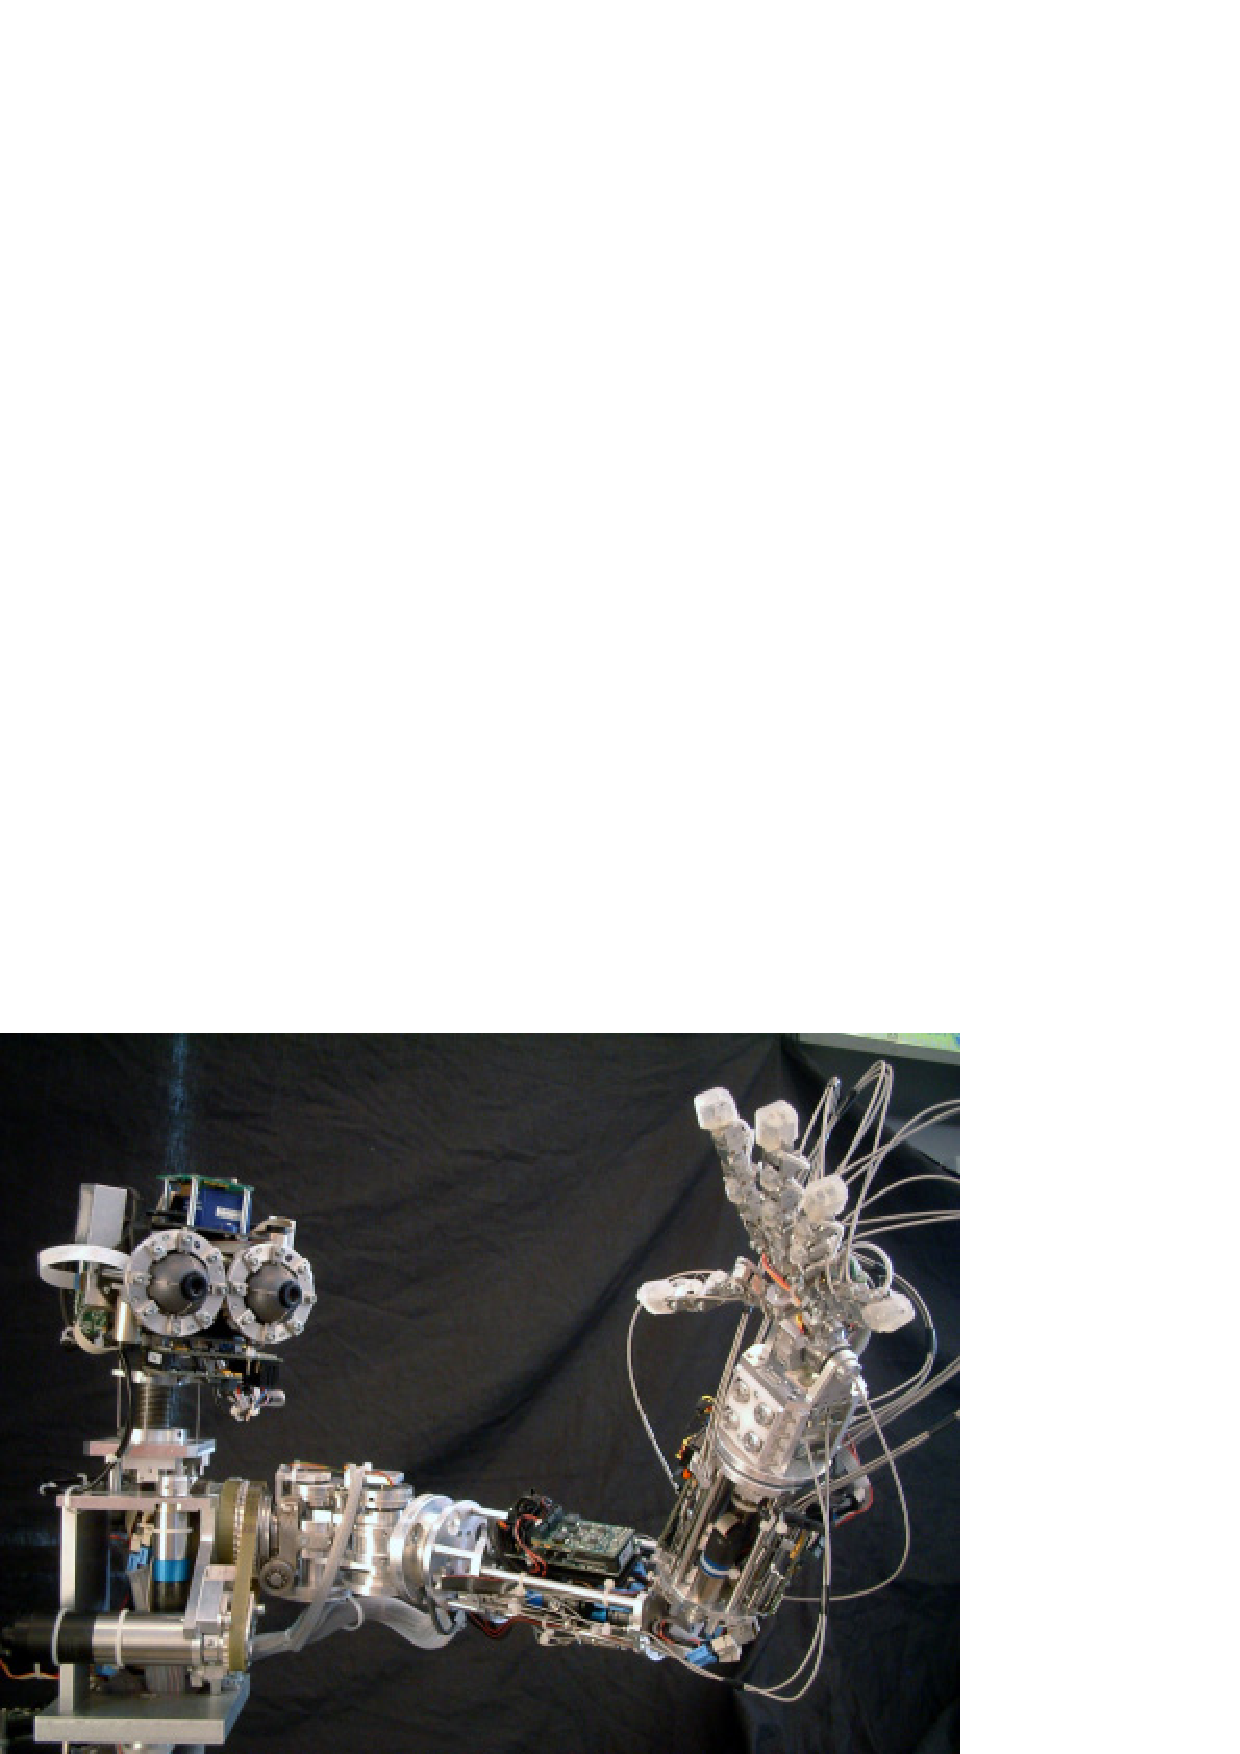
\includegraphics[width=50mm]{James1.png}
\caption{The humanoid robot James.}
\label{Fig:PicureJames}
\end{figure}

\subsection{Robot design}

The robot structure is similar to that of humans, both in size (approximatively that of a ten-year-old boy), number of DOFs and range of movements; the total weight (about 8 kg: 2 kg the head, 4 kg the torso and 2 kg arm and hand together) has been kept low by the employment of aluminum and Ergal.\\As already pointed out, such a complex structure is, in our view, mandatory when trying to replicate human-like movements on a humanoid robot.\\The head is equipped with two eyes, which can pan and tilt independently (4 DOFs), and is mounted on the 3-DOF neck, which allows the movement of the head as needed in the 3D rotational space.\\The arm has 7 DOFs: three of them are located in the shoulder, one in the elbow and three in the wrist. The hand has five fingers, with complexively 17 degrees of freedom, underactuated by just 8 motors.


\subsection{Actuation system}

The 22 DOFs are actuated by a total of 23 motors, whose torque is transmitted to the joints by plastic toothed belts and stainless-steel tendons, provided with springs at critical locations.\\This solution is appealing for at least two reasons. First, it allows to put the motors far from the joints, and so to distribute the weights within the robot in a smart way (i.e. put the heaviest motors on the static parts, like the torso). Second, the intrinsic elesticity of belts, tendons and springs gives a noteworthy compliance to the whole structure, as humans have, allowing the robot to move safely in a dynamic and unknown environment.

\subsection{Sensory system}

The robot is equipped with vision, proprioception, kinesthetic and tactile inputs.\\Vision is provided by two digital CCD cameras (PointGrey Dragonfly remote head), located in the eyeballs.\\The proprioceptive and kinesthetic senses are achieved through position sensors (magnetic incremental encoders connected to all motors and absolute-position sensors on the shoulder and in the fingers); furthermore, a 3-axis inertial sensor (Intersense iCube2) has been mounted on top of the head, to emulate the vestibular system.\\Tactile information is extracted from several magnetic silicone-made pressure sensors which have been specifically designed and developed for James, placed in the fingers.



\section{Neck structure} \label{Sec:NeckStructure}

The neck is actually constituted by a steel spring, which holds the head giving it the possiblity to rotate over three orthogonal axes.\\One motor directly actuates the head yaw (i.e. rotation around an axe parallel to the pan axes of the two eyes). The remaining three motors are arranged in a parallel configuration, and actuate the head's two additional rotations: pitch (i.e. rotation around an axe parallel to the tilt axes of the two eyes) and roll.\\These two rotations are achieved with an unconventional actuation system (see Figure \ref{Fig:HeadAct}). Each motor pulls a tendon; the tension of the three tendons determines the equilibrium configuration of the spring on which the head is mounted.\\The structure has an implicit compliance but it can become fairly stiff when needed by pulling the three tendons simultaneously.

\begin{figure}[tbp]
\centering
\includegraphics[width=50mm]{HeadAct.pdf} 
\caption{Neck actuation system. Each motor pulls a tendon in order to bring the spring (i.e. the neck) in the desired configuration.}
\label{Fig:HeadAct}
\end{figure}



\section{Control of the neck} \label{Sec:NeckControl}

The peculiar structure of the neck has required the design of an original control technique. The final design makes use of the 3-axis inertial sensor positioned on top of the robot head. The sensor measures the (absolute) pitch and roll rotations\footnote{The rotation is expressed by three angles which will be denoted roll ($\theta_r$), pitch ($\theta_p$) and yaw ($\theta_y$). The three motors of the neck influence the first two angles ($\theta_r$), pitch ($\theta_p$). The remaining degree of rotation ($\theta_y$) is directly influenced by the head pan which is moved by a specific motor.} of the head with respect to an inertial reference frame. Using the information from this sensor we developed a closed loop controller to orient the head in any desired configuration. 

\subsection{Neck control in details}

As already pointed out, the neck structure is characterized by three degrees of freedom: pitch $\theta_p$, roll $\theta_r$ and yaw $\theta_y$. The yaw movement, is directly actuated by a single dc motor; its control is based on a standard PID controller. The control strategy for the remaining two movements will be instead described in details in this section.

The design of the pitch and roll control loops has required the development of a \textsc{Matlab} model of the neck structure. The model is based on the assumption that the spring has a constant length\footnote{Practically, when the spring bends on a side, it maintains its length on that side while stretching on the opposite side. This kinematic can be easily modeled with \textsc{Matlab}.}. When the spring is bent, the assumption is that its curvature is constant along the entire spring length. Using this model we were able to compute the ideal tendons lengths given the pose of the neck, or equivalently the ideal tendons lengths ($l_1$, $l_2$, $l_3$) given the inertia sensor measurement ($\theta_r$, $\theta_p$). Practically, the model of the system is a function $f: \mathbb R^2 \longrightarrow \mathbb R^3$ such that:
\begin{eqnarray} \label{Eq:Model_neck}
\begin{bmatrix}
l_1\\
l_2\\
l_3
\end{bmatrix} = f (\theta_r, \theta_p).
\end{eqnarray}

The final control loop for positioning the neck in the desired configuration ($\theta_r^d$, $\theta_p^d$) is the following:
\begin{eqnarray} \label{Eq:Control_V1}
\begin{bmatrix}
\frac{d l_1}{dt}\\
\frac{d l_2}{dt}\\
\frac{d l_3}{dt}
\end{bmatrix} = -\begin{bmatrix} \frac{\partial f} {\partial \theta_r} &  \frac{\partial f} {\partial \theta_p} \end{bmatrix}
 \begin{bmatrix}
\theta_r - \theta_r^d\\
\theta_p - \theta_p^d
\end{bmatrix},
\end{eqnarray}
where $\begin{bmatrix} \frac{\partial f} {\partial \theta_r} &  \frac{\partial f} {\partial \theta_p} \end{bmatrix}$ is the Jacobian of the function $f$ with respect to $\theta_r$, $\theta_p$ computed at the current configuration $\theta_r$, $\theta_p$. 

The above model (\ref{Eq:Model_neck}) is ideal and assumes that the three tendons are always subject to a minimum tension. Due to the imperfections in the model, the tendons may loose tension if the control strategy (\ref{Eq:Control_V1}) is applied. Given a long enough time window the controller might drift. A corrective term is therefore required. The solution is:
\begin{eqnarray} \label{Eq:Control_V2}
\begin{bmatrix}
\frac{d l_1}{dt}\\
\frac{d l_2}{dt}\\
\frac{d l_3}{dt}
\end{bmatrix} = -(1-\gamma)\begin{bmatrix} \frac{\partial f} {\partial \theta_r} &  \frac{\partial f} {\partial \theta_p} \end{bmatrix}
 \begin{bmatrix}
\theta_r - \theta_r^d\\
\theta_p - \theta_p^d
\end{bmatrix} - \gamma \left( \begin{bmatrix} l_1\\
l_2\\
l_3
\end{bmatrix} - f(\theta_r, \theta_p) \right),
\end{eqnarray}
where $\gamma$ is an arbitrary constant in the range $[0, 1]$. The second term of the controller (the one multiplied by $\gamma$) guarantees that the the length of the cables remains similar to the length of the model. This strategy is sufficient to guarantee that the tendons maintain a tension which is more or less constant across different configurations of the structure. In this final configuration the jacobian $\begin{bmatrix} \frac{\partial f} {\partial \theta_r} &  \frac{\partial f} {\partial \theta_p} \end{bmatrix}$ can be substituted with a constant jacobian computed at the reference configuration $\theta_r$=$\theta_p$=0.


\section{Experimental data} \label{Sec:ExpData}


\section{Future work} \label{Sec:FutureWork}



\section{Conclusions} \label{Sec:Conclusions}





\bibliographystyle{plain}
\bibliography{MyBiblio}
\end{document}